% \centering
% /////////////////////////////////////////////////////////////////////
\chapter{Soket Programlama}

%----------------------------
\vspace{10mm}
\section{Giriş}
Soketler, aynı veya farklı makinelerdeki iki farklı işlem arasında iletişime izin verir. Daha kesin olmak gerekirse, standart Unix dosya tanımlayıcılarını kullanarak diğer bilgisayarlarla konuşmanın bir yolu. Unix'te her G/Ç eylemi, bir dosya tanıtıcısı yazılarak veya okunarak yapılır. Dosya tanımlayıcı yalnızca açık bir dosyayla ilişkili bir tamsayıdır ve bir ağ bağlantısı, metin dosyası, terminal veya başka bir şey olabilir.


\vspace{10mm}

\section{Soket Programlama Uygulama Alanları}

Bir istemci-sunucu uygulama çerçevesinde bir Unix Soketi kullanılır. Sunucu, bir istemciden gelen istek üzerine bazı işlevleri yerine getiren bir işlemdir. FTP, SMTP ve POP3 gibi uygulama düzeyindeki protokollerin çoğu, istemci ve sunucu arasında bağlantı kurmak ve ardından veri alışverişi için soketleri kullanır.
Soket Programlama TCP kullanarak istemci ve sunucu arasında bir bağlantı oluşturuyoruz, TCP yüksek güvenilirlik gerektiren uygulamalar için uygundur ve iletim süresi nispeten daha az kritiktir. HTTP, HTTPs, FTP, SMTP, Telnet gibi diğer protokoller tarafından kullanılır. TCP, veri paketlerini belirtilen sırada yeniden düzenler. Aktarılan verilerin bozulmadan kaldığına ve gönderildiği sırayla ulaştığına dair mutlak bir garanti vardır. TCP, Akış Kontrolü yapar ve herhangi bir kullanıcı verisi gönderilmeden önce bir soket bağlantısı kurmak için üç paket gerektirir. TCP, güvenilirlik ve tıkanıklık kontrolünü ele alır. Ayrıca hata denetimi ve hata kurtarma da yapar. Hatalı paketler kaynaktan hedefe yeniden iletilir.
\vspace{10mm}

% ///////////////////////////////////////////////////////////////////
\newpage
\section{OSI Katmanları}
\begin{figure}[!htb]
    \centering
    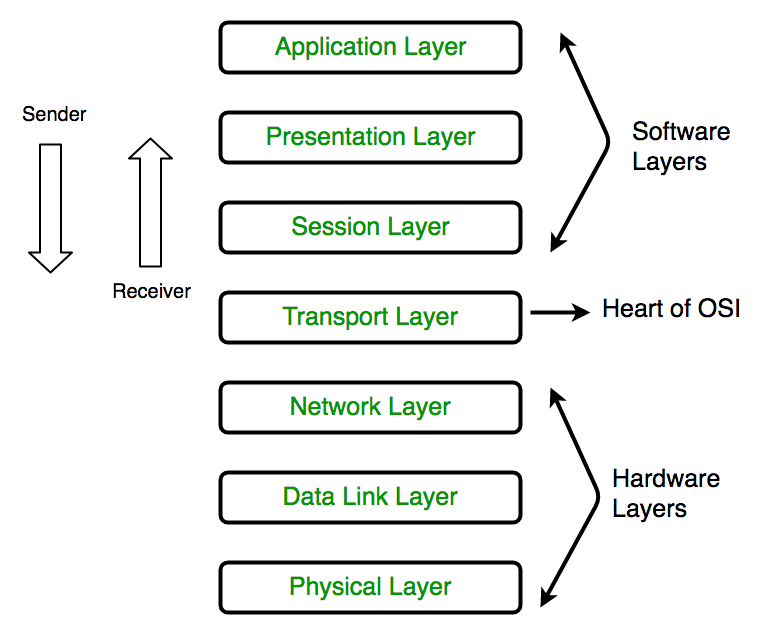
\includegraphics[width=1\linewidth]{00-images/08-osi_layers.png}
    \caption{OSI Katmanları}
    \label{fig:my_label}
\end{figure}


\vspace{10mm}
\textbf{1. Fiziksel Katman}
\vspace{5mm}

Fiziksel katman, ağ düğümleri arasındaki fiziksel kablo veya kablosuz bağlantıdan sorumludur. Cihazları bağlayan konektörü, elektrik kablosunu veya kablosuz teknolojiyi tanımlar ve bit hızı kontrolü ile ilgilenirken, sadece bir dizi 0 ve 1 olan ham verilerin iletilmesinden sorumludur.

\vspace{10mm}
\textbf{2. Veri Bağlantı Katmanı}
\vspace{5mm}

Veri bağlantı katmanı, bir ağ üzerinde fiziksel olarak bağlı iki düğüm arasında bir bağlantı kurar ve sonlandırır. Paketleri çerçevelere böler ve kaynaktan hedefe gönderir. Bu katman iki bölümden oluşur: Ağ protokollerini tanımlayan, hata denetimi gerçekleştiren ve çerçeveleri senkronize eden Mantıksal Bağlantı Kontrolü (LLC) ve cihazları bağlamak ve veri iletmek ve almak için izinleri tanımlamak için MAC adreslerini kullanan Medya Erişim Kontrolü (MAC).

\vspace{10mm}
\textbf{3. Ağ Katmanı}
\vspace{5mm}

Ağ katmanının iki ana işlevi vardır. Biri, segmentleri ağ paketlerine bölmek ve paketleri alıcı uçta yeniden birleştirmek. Diğeri ise paketleri fiziksel bir ağ üzerinde en iyi yolu keşfederek yönlendirmektir. Ağ katmanı, paketleri bir hedef düğüme yönlendirmek için ağ adreslerini (tipik olarak İnternet Protokolü adresleri) kullanır.

\vspace{10mm}
\textbf{4. Taşıma Katmanı}
\vspace{5mm}

Taşıma katmanı, oturum katmanında aktarılan verileri alır ve iletim tarafında “bölümlere” ayırır. Alıcı taraftaki segmentleri yeniden birleştirmek ve oturum katmanı tarafından kullanılabilecek verilere dönüştürmekten sorumludur. Taşıma katmanı, akış kontrolünü, alıcı cihazın bağlantı hızına uygun bir hızda veri gönderme ve hata kontrolünü, verinin yanlış alınıp alınmadığını kontrol edip, değilse tekrar talep ederek gerçekleştirir.

\vspace{10mm}
\textbf{5. Oturum Katmanı}
\vspace{5mm}

Oturum katmanı, cihazlar arasında oturum adı verilen iletişim kanalları oluşturur. Oturumların açılmasından, veriler aktarılırken açık ve işlevsel kalmasının sağlanmasından ve iletişim sona erdiğinde kapatılmasından sorumludur. Oturum katmanı ayrıca veri aktarımı sırasında kontrol noktaları ayarlayabilir; oturum kesilirse cihazlar son kontrol noktasından veri aktarımına devam edebilir.

\vspace{10mm}
\textbf{6. Sunum Katmanı}
\vspace{5mm}

Sunum katmanı, uygulama katmanı için verileri hazırlar. Diğer uçta doğru şekilde alınması için iki cihazın verileri nasıl kodlaması, şifrelemesi ve sıkıştırması gerektiğini tanımlar. Sunum katmanı, uygulama katmanı tarafından iletilen herhangi bir veriyi alır ve oturum katmanı üzerinden aktarım için hazırlar.

\vspace{10mm}
\textbf{7. Uygulama Katmanı}
\vspace{5mm}

Uygulama katmanı, web tarayıcıları ve e-posta istemcileri gibi son kullanıcı yazılımları tarafından kullanılır. Yazılımın bilgi gönderip almasına ve kullanıcılara anlamlı veriler sunmasına izin veren protokoller sağlar. Uygulama katmanı protokollerine birkaç örnek, Hypertext Transfer Protocol (HTTP), File Transfer Protocol (FTP), Post Office Protocol (POP), Simple Mail Transfer Protocol (SMTP), Domain Name System (DNS).

% ///////////////////////////////////////////////////////////////////

\vspace{20mm}
\section{TCP/UDP Protokolleri}
\begin{figure}[!htb]
    \centering
    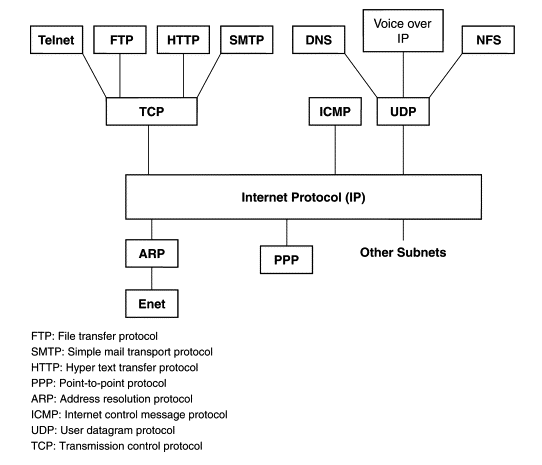
\includegraphics[width=1\linewidth]{00-images/11-network.png}
    \caption{TCP/UDP Protokolleri}
    \label{fig:my_label}
\end{figure}

\vspace{10mm}
\textbf{İnternet Protokolü}
\vspace{5mm}

Genel olarak konuşmak gerekirse internet birbirine bağlanan cihazlar bütünüdür. Akıllı telefonunuz, kişisel bilgisayarınız veya sunucunuz olsun, her cihaz internet protokol paketi aracılığıyla iletişim kurar. İnternet protokol paketi, cihazların birbirleriyle iletişim kurması için farklı protokoller veya yöntemler topluluğudur. Hem TCP hem de UDP, internet protokol paketindeki ana protokollerdir. İnternete bağlı her cihazın benzersiz bir IP adresi vardır. Herhangi iki cihaz internet protokolü üzerinden iletişim kurmak isterse TCP veya UDP protokolünü kullanır.

\begin{figure}[!htb]
    \centering
    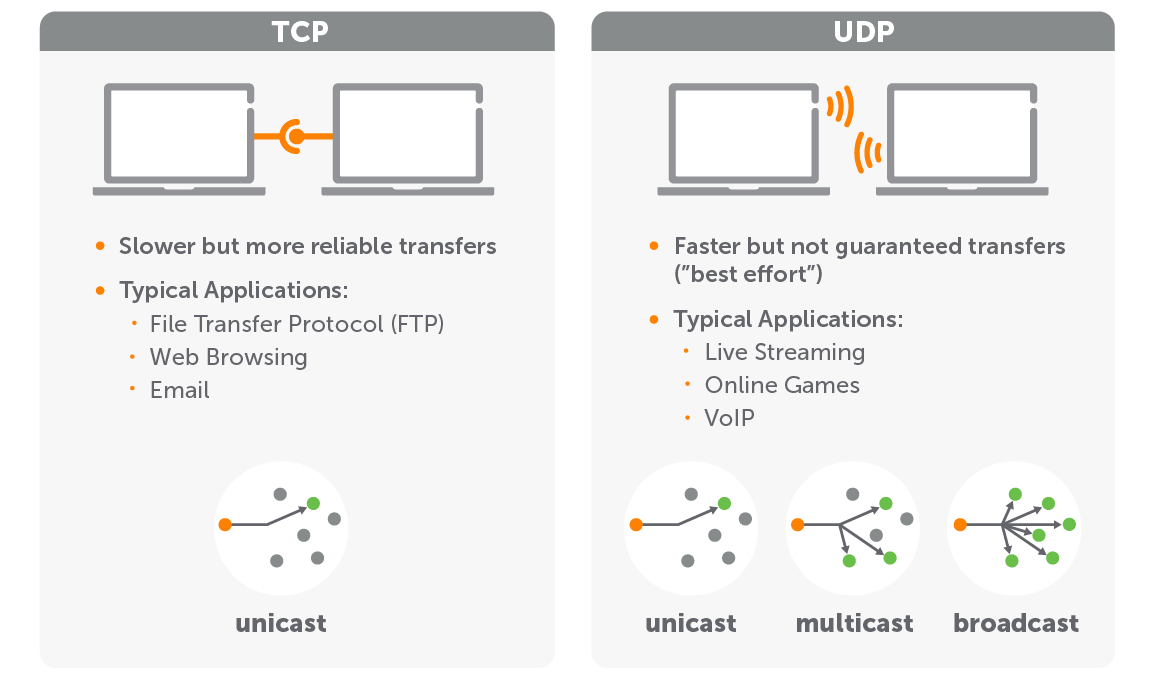
\includegraphics[width=1\linewidth]{00-images/12-tcp_udp.png}
    \caption{TCP/UDP Protokol Karşılaştırılması}
    \label{fig:my_label}
\end{figure}

\vspace{10mm}
\textbf{TCP Protokolü}
\vspace{5mm}

TCP veya İletim Kontrol Protokolü (Transmission Control Protocol), çevrimiçi olarak en yaygın ağ protokolüdür. TCP son derece güvenilirdir ve internette gezinmeye (HTTP), e-posta göndermeye (SMTP) ve dosya aktarmaya (FTP) kadar her şey için kullanılır.
TCP, bir cihaz tarafından gönderilen tüm verilerin başka bir cihaz tarafından tamamen bozulmamış olarak alınmasının gerekli olduğu durumlarda kullanılır.
Örneğin, bir web sitesini ziyaret ettiğinizde, sayfayı oluşturmak için gereken metin, resim ve koddaki her şeyin size ulaştığını garanti etmek için TCP kullanılır. TCP olmadan, resimler veya metinler eksik olabilir veya yanlış sırada gelerek sayfayı bozabilir.
TCP, bağlantı yönelimli bir protokoldür, yani veri aktarmadan önce iki cihaz arasında bir bağlantı kurar ve aktarım işlemi boyunca bu bağlantıyı korur.
TCP, iki cihaz arasında bağlantı kurmak için üç yönlü handshake adı verilen bir yöntem kullanır.


\begin{figure}[!htb]
    \centering
    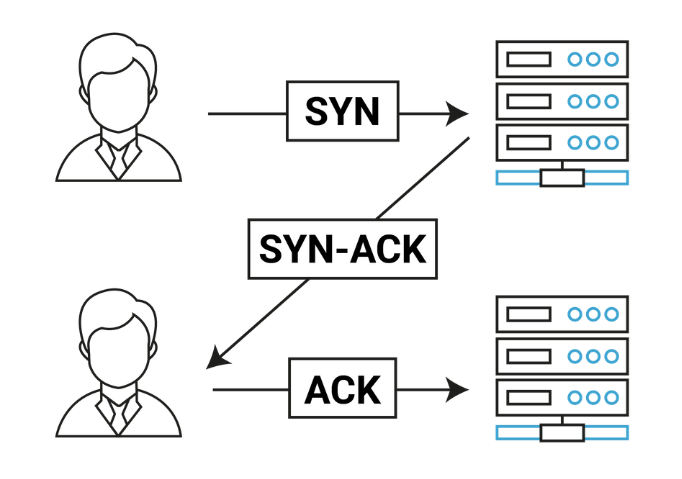
\includegraphics[width=1\linewidth]{00-images/13-tcp.png}
    \caption{Üç Yönlü Handshake}
    \label{fig:my_label}
\end{figure}

\vspace{10mm}
\textbf{Üç Yönlü Handshake}
\vspace{5mm}

Örneğin, cihazınızda bir haber okumak için cihazınız önce SYN (Senkronizasyon Sıra Numarası) adlı o Haber Sitesinin Sunucusuna bir mesaj gönderir. 
Ardından Haber Sitesinin Sunucusu, SYN-ACK adı verilen bir onay mesajını geri gönderir.
Cihazınız sunucudan SYN-ACK aldığında, bağlantıyı kuran bir ACK onay mesajı gönderir.
İki cihaz arasında bir TCP bağlantısı kurulduğunda, protokol tüm verilerin iletilmesini garanti eder.
Cihazınız ve Haber Sitesi örneğine geri dönersek, üç yönlü anlaşma tamamlandıktan sonra Haber Sitesinin Sunucusu, cihazınızın web tarayıcısının makaleyi oluşturmak için ihtiyaç duyduğu tüm verileri göndermeye başlayabilir.
Tüm cihazlar, verileri internet üzerinden göndermeden önce küçük paketlere ayırır. Bu paketlerin daha sonra diğer uçta yeniden birleştirilmesi gerekir.
Bu nedenle, Haber Sitesinin Sunucusu bu makale için HTML, CSS, Resimler ve diğer Kodları gönderdiğinde, bunları cihazınıza göndermeden önce her şeyi küçük veri paketlerine böler. Cihazınız daha sonra bu paketleri, bu makaleyi oluşturmak için ihtiyaç duyduğu dosyalara ve görüntülere yeniden birleştirir.
TCP, bu paketlerin tümünün cihazınıza ulaşmasını sağlar. Yol boyunca herhangi bir paket kaybolursa, TCP, cihazınızın sunucunun eksik veri olduğunu bilmesini ve sunucunun bu paketleri yeniden göndermesini kolaylaştırır.
Cihazınız makaleyi oluşturmak için ihtiyaç duyduğu tüm verileri aldığında, TCP, bu sefer FIN ve ACK paketlerini kullanarak üç yönlü Handshake benzer bir yöntemle iki cihaz arasındaki bağlantıyı otomatik olarak sonlandırır.

\vspace{15mm}

\begin{figure}[!htb]
    \centering
    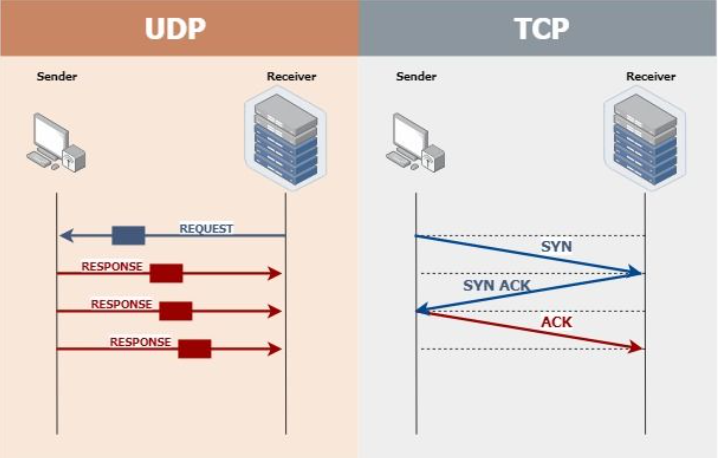
\includegraphics[width=1\linewidth]{00-images/14-tcp_udp.png}
    \caption{TCP/UDP Protokol Farkları}
    \label{fig:my_label}
\end{figure}


\vspace{10mm}
\textbf{UDP Protokolü}
\vspace{5mm}

UDP veya Kullanıcı Datagram Protokolü (User Datagram Protocol), internet protokol paketini oluşturan ana protokollerden bir diğeridir. UDP, TCP'den daha az güvenilirdir, ancak çok daha basittir.
UDP, canlı video/ses gibi bazı veri kayıplarının kabul edilebilir olduğu veya çevrimiçi oyunlar gibi hızın kritik bir faktör olduğu durumlarda kullanılır.
UDP, çevrimiçi veri göndermek ve almak için kullanıldığı için TCP'ye benzer olsa da, birkaç önemli fark vardır.
Birincisi, UDP bağlantısız bir protokoldür, yani TCP'nin üç yönlü handshake ile yaptığı gibi önceden bir bağlantı kurmaz.
Ardından, UDP tüm verilerin başarıyla aktarıldığını garanti etmez. UDP ile, dinlemeye başlayan herhangi bir cihaza veri gönderilir, ancak bir kısmının yolda kaybolması umurunda değildir. UDP'nin "ateşle ve unut" (fire and forget) protokolü olarak da bilinmesinin nedenlerinden biri de budur.
Bu farklılıklar hakkında düşünmenin iyi bir yolu, TCP'nin iki kişi arasındaki bir konuşma gibi olmasıdır. A kişisi B kişisinden konuşmasını ister. B kişisi kabul eder ve ikisi de konuşmaya başlar.
UDP daha çok dışarıda megafonlu bir satıcıya benzer. Satıcıya dikkat eden herkes, söylediklerinin çoğunu duyabilir. Ancak bölgedeki herkesin Satıcının söylediklerini duyacağının veya hatta dinlediklerinin garantisi yoktur.

\vspace{10mm}

% ///////////////////////////////////////////////////////////////////

\section{İnternet Protokolü ve Portlar}

\vspace{5mm}
\textbf{İnternet Protokolü}
\vspace{5mm}

İnternet Protokolü (IP), ağlar arasında transfer edilebilmeleri ve doğru hedefe varabilmeleri için veri paketlerini yönlendirmek ve adreslemek için bir protokol veya kurallar dizisidir. İnternette dolaşan veriler, paket adı verilen daha küçük parçalara bölünür. Her pakete IP bilgisi eklenir ve bu bilgi yönlendiricilerin paketleri doğru yere göndermesine yardımcı olur. İnternete bağlanan her cihaza veya etki alanına bir IP adresi atanır ve paketler bunlara bağlı IP adresine yönlendirildikçe veriler ihtiyaç duyulan yere ulaşır. Paketler hedeflerine ulaştığında, IP ile birlikte hangi taşıma protokolünün kullanıldığına bağlı olarak farklı şekilde işlenirler. En yaygın aktarım protokolleri TCP ve UDP'dir.

\vspace{10mm}
\textbf{İnternet Protokol Versiyon 4}
\vspace{5mm}

İnternet Protokolü Versiyon 4 (IPv4), İnternet Protokolünün (IP) dördüncü sürümüdür. İnternette ve diğer paket anahtarlamalı ağlarda standartlara dayalı ağlar arası çalışma yöntemlerinin temel protokollerinden biridir. IPv4, 1982'de SATNET'te ve Ocak 1983'te ARPANET'te üretim için dağıtılan ilk sürümdü. Bugün hala çoğu İnternet trafiğini yönlendirmek için kullanılıyor.
IPv4, 4,294,967,296 $(2^{32})$ benzersiz adres sağlayan 32 bitlik bir adres alanı kullanır, ancak büyük bloklar özel ağ oluşturma amaçları için ayrılmıştır.

\begin{figure}[!htb]
    \centering
    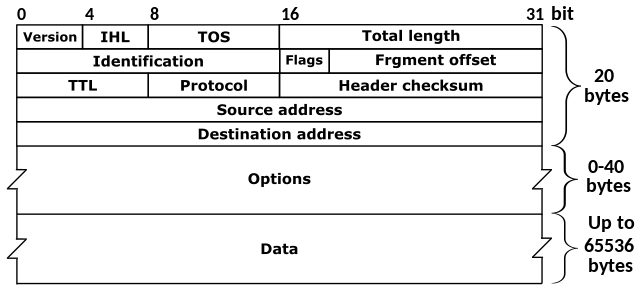
\includegraphics[width=1\linewidth]{00-images/10-internet_protocol_v4.png}
    \caption{Internet Protokol Versiyon 4}
    \label{fig:my_label}
\end{figure}

\vspace{10mm}
\textbf{İnternet Protokol Versiyon 6}
\vspace{5mm}

İnternet Protokolü sürüm 6 (IPv6), ağlardaki bilgisayarlar için bir tanımlama ve konum sistemi sağlayan ve trafiği İnternet üzerinden yönlendiren iletişim protokolü olan İnternet Protokolü'nün (IP) en son sürümüdür. IPv6, Internet Engineering Task Force (IETF) tarafından uzun zamandır beklenen IPv4 adres tükenmesi sorunuyla başa çıkmak için geliştirildi ve IPv4'ün yerini alması amaçlandı. Aralık 1998'de IPv6, IETF için Taslak Standart oldu ve daha sonra 14 Temmuz 2017'de bir İnternet Standardı olarak onaylandı. IPv6, 340,282,366,920,938,463,463,374,607,431,768,211,456 $(2^{128})$ benzersiz adres sağlayan 128 bitlik bir adres alanı kullanır.

\begin{figure}[!htb]
    \centering
    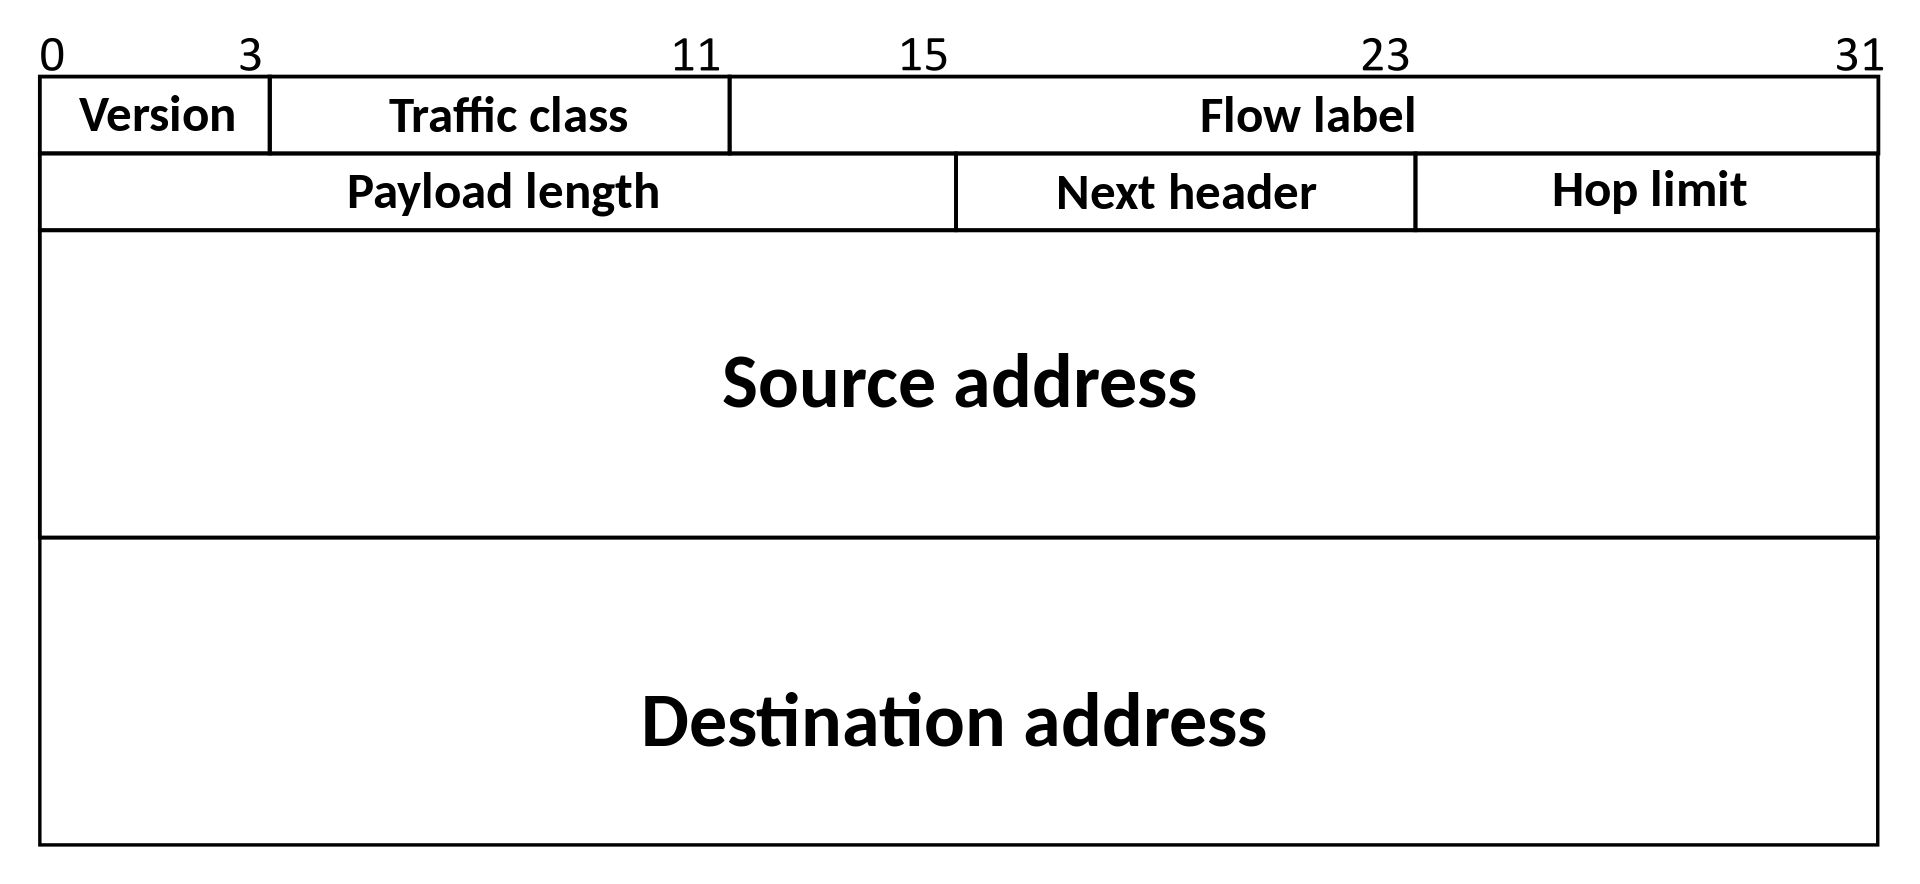
\includegraphics[width=1\linewidth]{00-images/10-internet_protocol_v6.png}
    \caption{Internet Protokol Versiyon 6}
    \label{fig:my_label}
\end{figure}

\newpage

\vspace{10mm}
\textbf{IPv4 ve IPv6 Karşılaştırılması}
\vspace{5mm}

\begin{figure}[!htb]
    \centering
    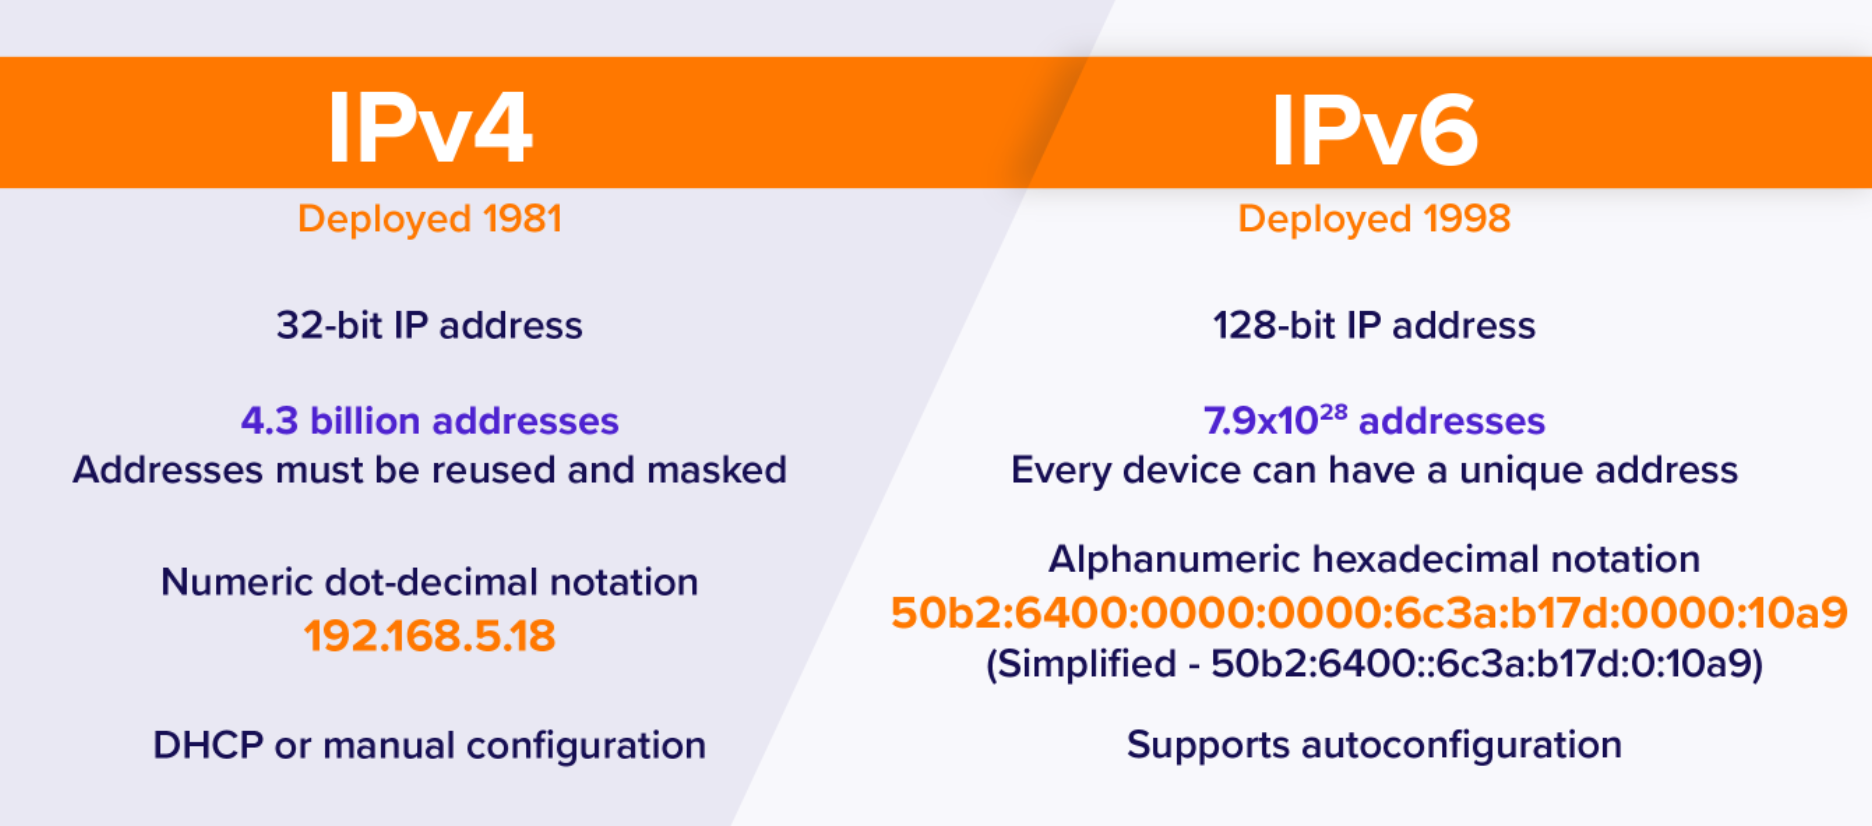
\includegraphics[width=1\linewidth]{00-images/15-ipv4_vs_ipv6.png}
    \caption{IPv4 ve IPv6 Karşılaştırılması}
    \label{fig:my_label}
\end{figure}

\begin{figure}[!htb]
    %
    \centering
    \subfloat[\centering IPv4 Header]{{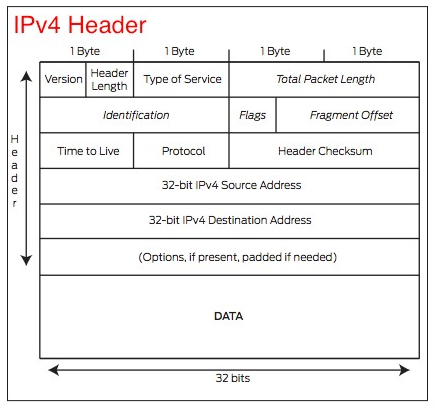
\includegraphics[width=6.6cm]{00-images/15-ipv4_header.png} }}%
    \qquad
    \subfloat[\centering IPv6 Header]{{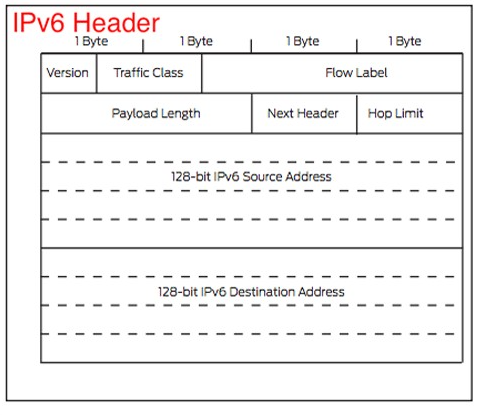
\includegraphics[width=7cm]{00-images/15-ipv6_header.png} }}%
    \caption{IPv4 ve IPv6 Header Karşılaştırılması}%
    \label{fig:example}
    %
\end{figure}



\newpage

\vspace{10mm}
\textbf{Portlar}
\vspace{5mm}

Port numarası, bilgisayar ağlarında mesajların göndericilerini ve alıcılarını tanımlamak için kullanılan adresleme bilgilerinin bir parçasıdır. Gelen trafiğin hangi protokole yönlendirileceğini belirlemek için farklı port numaraları kullanılır. Bağlantı noktası numarası, bir İnternet veya başka bir ağ mesajının bir sunucuya ulaştığında iletileceği belirli bir işlemi tanımlar. Her protokol için bağlantı noktaları tanımlanır ve bir iletişim uç noktası olarak kabul edilir.

Bağlantı noktaları 16 bitlik sayılarla temsil edilir. 65336  $(2^{16})$ bağlantı noktası numarası vardır.

\vspace{10mm}
\textbf{Port Grupları}
\vspace{5mm}

0 ila 1023 - İyi bilinen (Well Known) port numaraları. Yalnızca Apple QuickTime, MSN, SQL Services, Gopher Services ve diğer önde gelen hizmetler gibi özel şirketler bu bağlantı noktası numaralarına sahiptir.

1024 - 49151 - Kayıtlı bağlantı noktaları (Registered Ports); Yazılım şirketleri tarafından belirli protokollere kaydedilirler.

49152 ila 65536 - Dinamik veya özel bağlantı noktaları (Dynamic or Private ports); Hemen hemen herkes tarafından kullanılabilirler.


\vspace{20mm}
\textbf{Soket}
\vspace{5mm}

Bir uygulama, IP adresi ve bağlantı noktası(Port) numarasının birleşimini bilerek TCP/IP ile remote bir işlem aracılığıyla iletişim kurabilir. Bu kombinasyon genellikle soket adresi olarak bilinir.

\begin{figure}[!htb]
    \centering
    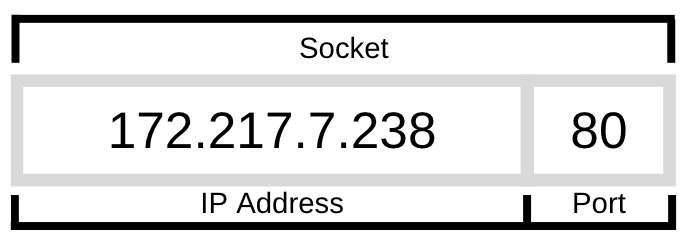
\includegraphics[width=1\linewidth]{00-images/15-socket_address.png}
    \caption{Soket Adresi}
    \label{fig:my_label}
\end{figure}

% ///////////////////////////////////////////////////////////////////

\section{TCP Soket Server ve Client}

\begin{question}
TCP Soket kullanılarak Kullanıcı\textbf{(Client)} tarafından input olarak alınan tek seferlik mesajın Sunucuya\textbf{(Server)} aktarılmasını sağlıyan sistem için:
	\\ a) Uygun TCP Socket Serveri Tasarlayınız.
	\\ b) Uygun TCP Socket Clienti Tasarlayınız. 
\end{question}

a) TCP Socket Server
\vspace{2mm}
\lstinputlisting[language=Go]{codes/11-tcp_socket_server.go }
\captionof{table}{TCP Soket Server}

b) TCP Socket Client
\vspace{2mm}
\lstinputlisting[language=Go]{codes/11-tcp_socket_server.go }
\captionof{table}{TCP Soket Client}

% ///////////////////////////////////////////////////////////////////

\section{TCP Socketi Ile Surekli İletişim Sağlanması}

\begin{question}
TCP Socket kullanılarak Tek Kullanıcı\textbf{(Client)} tarafından input olarak alınan ve bağlantı süresince birden fazla gönderilebilen mesajın Sunucu\textbf{(Server)} tarafından sürekli olarak karşılanmasını sağlayan sistem için:
	\\ a) Uygun TCP Socket Serveri Tasarlayınız.
	\\ b) Uygun TCP Socket Clienti Tasarlayınız.
\end{question}


a) TCP Socket Server
\lstinputlisting[language=Go]{codes/12-tcp_socket_server.go }
\captionof{table}{TCP Soket Server}

b) TCP Socket Client
\lstinputlisting[language=Go]{codes/12-tcp_socket_server.go }
\captionof{table}{TCP Soket Client}

% ///////////////////////////////////////////////////////////////////
\vspace{20mm}

\section{TCP Socket Serverin Goroutinelerle Birden Fazla Clienti Karsilamasi}

\begin{question}
TCP Socket kullanılarak birden fazla Kullanıcı\textbf{(Client)} tarafından input olarak alınan ve bağlantı süresince birden fazla gönderilebilen mesajın Sunucu\textbf{(Server)} tarafından sürekli olarak karşılanmasını sağlayan sistem için:
	\\ a) Uygun TCP Socket Serveri Tasarlayınız.
	\\ b) Uygun TCP Socket Clienti Tasarlayınız.
\end{question}

a) TCP Socket Server
\lstinputlisting[language=Go]{codes/13-tcp_socket_server.go }
\captionof{table}{TCP Soket Server}

b) TCP Socket Client
\lstinputlisting[language=Go]{codes/13-tcp_socket_server.go }
\captionof{table}{TCP Soket Client}

% ///////////////////////////////////////////////////////////////////

\section{UDP Socketi}

\begin{question}
UDP Soket kullanılarak Kullanıcı\textbf{(Client)} tarafından input olarak alınan tek seferlik mesajın Sunucuya\textbf{(Server)} aktarılmasını sağlıyan sistem için:
	\\ a) Uygun UDP Socket Serveri Tasarlayınız.
	\\ b) Uygun UDP Socket Clienti Tasarlayınız.  
\end{question}

\lstinputlisting[language=Go]{codes/14-udp_socket_server.go }
\captionof{table}{UDP Soket Server}

\lstinputlisting[language=Go]{codes/14-udp_socket_client.go }
\captionof{table}{UDP Soket Client}

% ///////////////////////////////////////////////////////////////////

\section{UDP Socket Servera Çoklu Client Bağlantısı}

\begin{question}
UDP Socket kullanılarak birden fazla Kullanıcı\textbf{(Client)} tarafından input olarak alınan ve birden fazla gönderilebilen mesajın Sunucu\textbf{(Server)} tarafından sürekli olarak karşılanmasını sağlayan sistem için:
	\\ a) Uygun UDP Socket Serveri Tasarlayınız.
	\\ b) Uygun UDP Socket Clienti Tasarlayınız. 
\end{question}


\lstinputlisting[language=Go]{codes/15-udp_socket_server.go }
\captionof{table}{UDP Soket Server}

\lstinputlisting[language=Go]{codes/15-udp_socket_client.go }
\captionof{table}{UDP Soket Client}

% ///////////////////////////////////////////////////////////////////
% needs to be fixed
% \section{UDP Socketi Uzerinden Guvenli Veri Akisi Saglanmasi }

% \begin{question}
% UDP Socket Kullanılarak Veri Aktarımı İçin:
% 	\\ a) Server .
% 	\\ b) Client . 
% \end{question}

% \lstinputlisting[language=Go]{00-codes/16-udp_socket_server.go }
% \captionof{table}{UDP Soket Server}

% \lstinputlisting[language=Go]{00-codes/16-udp_socket_client.go }
% \captionof{table}{UDP Soket Client}

% ///////////////////////////////////////////////////////////////////

\section{Port Taramasi}

\begin{question}
Sistemde açık olarak bulunan portların taranması için:
	\\ a) Uygun TCP Port Taraması Sciptini Yazınız.
	\\ b) Uygun UDP Port Taraması Sciptini Yazınız. 
\end{question}

\lstinputlisting[language=Go]{codes/17-port_scanner.go }
\captionof{table}{UDP ve TCP Port Taraması}


% ///////////////////////////////////////////////////////////////////
% needs to be fixed
% \section{TCP Proxy Server Olusturulmasi}

% \begin{question}
% TCP Proxy:
% 	\\ a) Server .
% \end{question}

% \lstinputlisting[language=Go]{00-codes/18-proxy_server.go }

% \captionof{table}{TCP Proxy Server}

% ///////////////////////////////////////////////////////////////////
